%課題研究レジュメテンプレート ver. 1.2

\documentclass[uplatex]{jsarticle}
\usepackage[top=20mm,bottom=20mm,left=20mm,right=20mm]{geometry}
\usepackage[T1]{fontenc}
\usepackage{txfonts}
\usepackage{wrapfig}
\usepackage[expert,deluxe]{otf}
\usepackage[dvipdfmx,hiresbb]{graphicx}
\usepackage[dvipdfmx]{hyperref}
\usepackage{pxjahyper}
\usepackage{secdot}

\makeatletter
  \renewcommand{\section}{%
    \if@slide\clearpage\fi
    \@startsection{section}{1}{\z@}%
    {\Cvs \@plus.5\Cdp \@minus.2\Cdp}% 前アキ
    {.5\Cvs \@plus.3\Cdp}% 後アキ
    %{\normalfont\Large\headfont\raggedright}}
    {\normalfont\raggedright}}

  \renewcommand{\subsection}{\@startsection{subsection}{2}{\z@}%
    {\Cvs \@plus.5\Cdp \@minus.2\Cdp}% 前アキ
    {.5\Cvs \@plus.3\Cdp}% 後アキ
    %{\normalfont\large\headfont}}
    {\normalfont}}

  \renewcommand{\subsubsection}{\@startsection{subsubsection}{3}{\z@}%
    {\Cvs \@plus.5\Cdp \@minus.2\Cdp}%
    {\z@}%
    %{\normalfont\normalsize\headfont}}
    {\normalfont}}
\makeatother
%ここから上を編集する必要はない.





\title{\vspace{-14mm}上位下位関係抽出ツールを使用した語彙変換システム}
\author{PMコース 矢吹研究室 1342069 下村 渉}
\date{}%日付を入れる必要はない.
\pagestyle{empty}%ページ番号は振らない.
\begin{document}
\maketitle





\section{研究の背景}

プロジェクトの進行に密接に関わってくる環境的・技術的などの要因は多々あるが,最も重要な事は関係者間のコミュニケーションである.コミュニケーションを重要視して適切に取っていく事は,どのような効果が期待できるか.それは,関係者間での認識のズレ,使用の抜け・漏れ,誤解が生まれるのを防止するという効果がある.それにより,プロジェクトの円滑な進行が期待できる.発注者と開発者との間の「不適切なコミュニケーション」の例としては次のようなものが考えられる.
\begin{itemize}
  \item 開発者の専門的な用語を使った説明では,発注者は十分な理解を得られないかもしれない
  \item 発注者が「実装して当然」と想定している機能について,開発者は「開発者から何も言われていない」という理由で,実装する機能として想定していないかもしれない
  \end{itemize}

仕様書や設計書,計画書などのドキュメントを作る目的の一つとしては「関係者間のコミュニケーションツールとして利用するため」という事である.仕様書や設計書,計画書などのドキュメントは発注者の要求を開発者が十分に汲み取り,要件として落とし込めているか,要件に過不足は無いか,発注者と開発者の認識を合わせるためのツールであり,開発側内部では,詳細な設計や実装を行うエンジニアとのコミュニケーションツールにも利用されるだろう\cite{a}.

本研究では,発注者と開発者がそれぞれ使う専門的な用語を目的に応じた用語に変換を実現する共通な仕組みができないか着目し,用語の変換を行うために用語をタグで結び,関連用語を抽出することを考える.これと同じような事例を探し,参考に研究する.そして,2008年のWikipediaの記事構造から上位下位関係抽出の論文を参考にし,MediaWikiを利用する.\cite{b}
 
 MediaWikiは現在,オープンソース(GPL)で配布されているので,MediaWikiを利用すれば,自分専用のWikipediaを運用できる\cite{c}.MediaWikiを利用し,目的に応じて語彙の変換を可能にするシステムを研究する.





\section{研究の目的}

本研究では,MediaWiki内にある単語の上位下位関係を抽出し,関係者間での視点や用語が異なる語彙を目的に応じた最適な語彙への変換ができるようなシステムを作ること.また卒論で応用するため知識を深めるためである.





\section{プロジェクトマネジメントとの関連}

本研究は,発注者が発注する際に作る仕様書,設計書を開発者が十分に理解するためなどに使用する.これは発注者と開発者の不適切なコミュニケーションを避けることが出来るのでコミュニケーションマネジメントに関連づくと考えられる.







\section{研究の方法}

本研究ではMediaWikiのサーバーを立ち上げ,各視点から専門用語のページを作り,作ったページから用語間の関連情報を抽出し,抽出した情報から用語の翻訳する.










\section{現在の進捗状況}

現在の進捗状況はMediaWikiをインストールしていくつかページを作り,MediaWikiのデータをXMLにダンプし上位下位関係抽出ツールで解析し抽出した.抽出したデータを少しだけ紹介する.\\

\begin{figure}[htbp]
  \begin{center}
    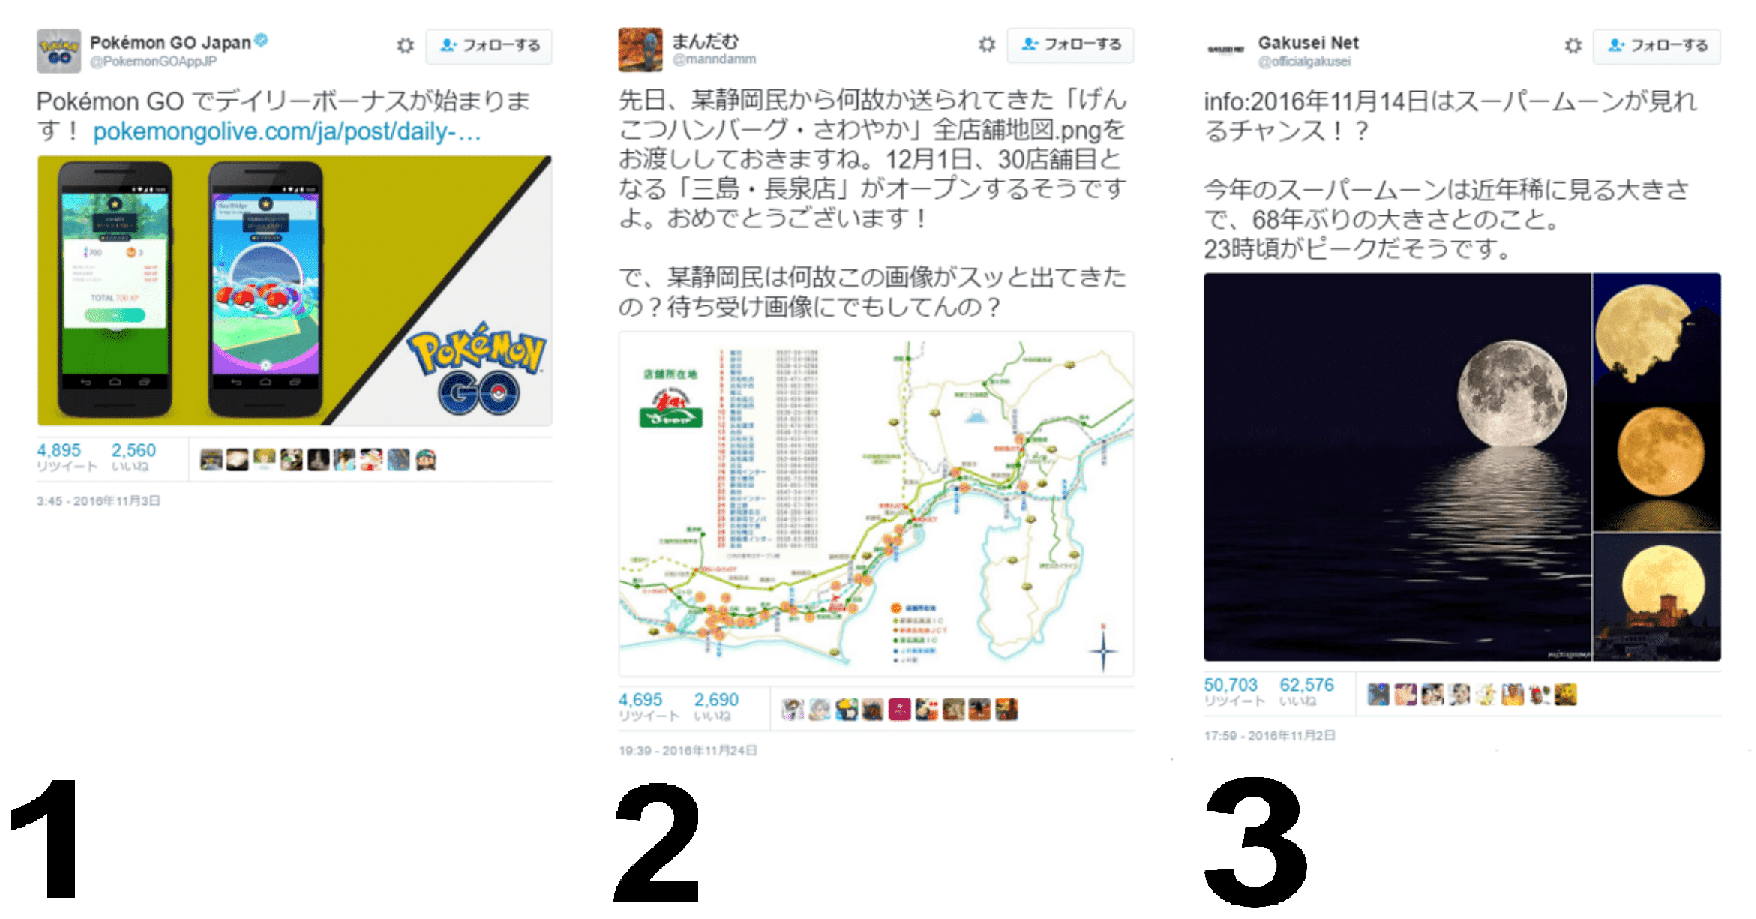
\includegraphics[clip,width=7.0cm]{g1.pdf}
    \label{fig:hamu}
  \end{center}
\end{figure}

この結果は「グランブルーファンタジー」というページの「メインキャラクター」の解析結果で,左から上位語,下位語,SVMを示している.
次に同じページの「登場キャラクター」の解析結果の一部を記載する.
\begin{figure}[htbp]
  \begin{center}
    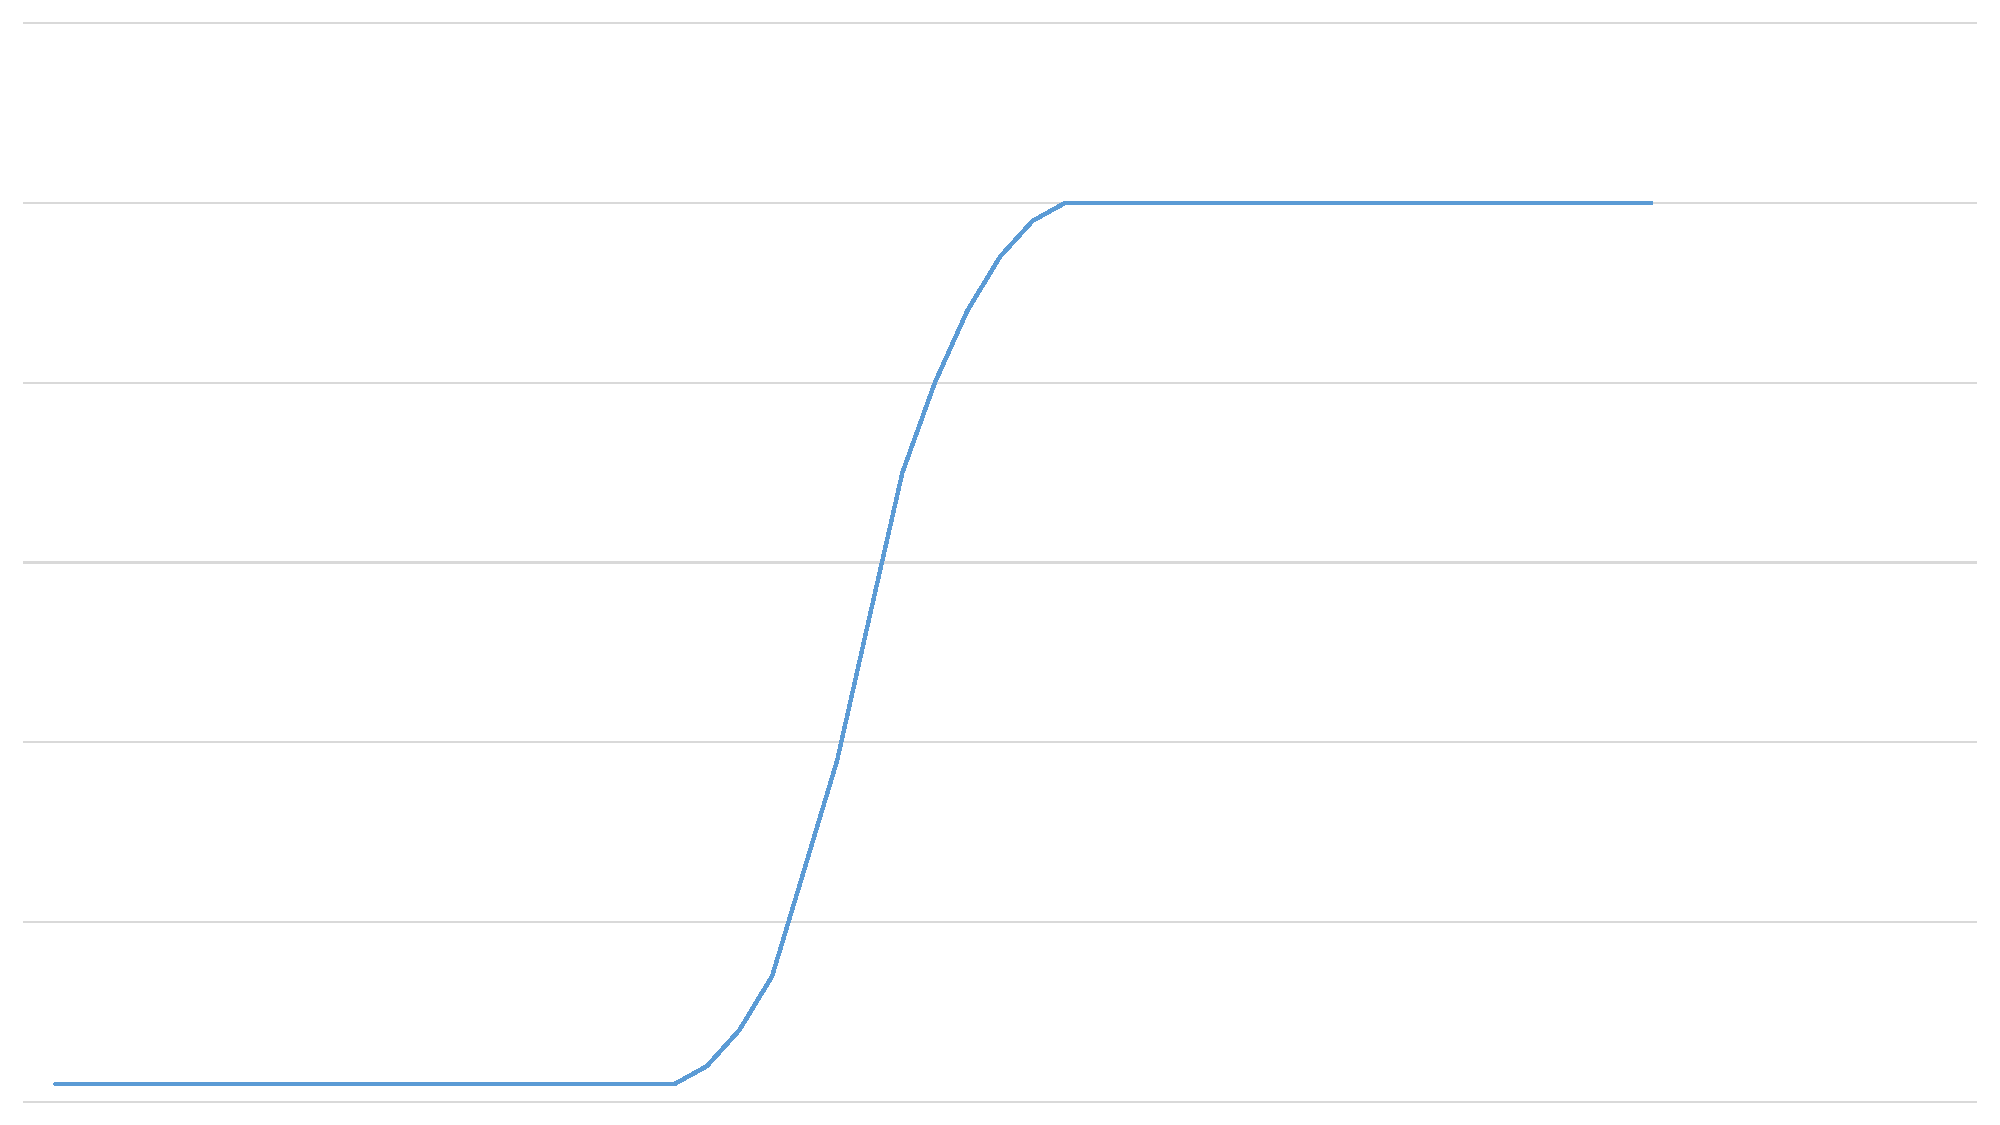
\includegraphics[clip,width=7.0cm]{g2.pdf}
    \label{fig:hamu}
  \end{center}
\end{figure}

記載した解析結果は「メインキャラクター」とそれ以外のキャラクターの結果を交互に並べたものである.この結果より「メインキャラクター」で抽出されたキャラはSVMが1.3を超えていてそうでないキャラクターは基本下回っていることが分かるが,たまに上回っているものもある.



\section{今後の計画}


今後の計画は専門用語を検索したときに適切な用語に転換できるよう検索システムの開発を予定している.


\bibliographystyle{junsrt}
\bibliography{biblio}%「biblio.bib」というファイルが必要.

\end{document}
